% ============================================================
% FUENTES: body/body.tex; Notas Biomate 1; raw_plain_nonlinear_dynamics.txt.
% Murray (2002); Strogatz (2015), caps. 6 y 7; Edelstein-Keshet (2007).
% ============================================================
\section{El modelo de Lotka--Volterra y ciclos límite}

En este capítulo analizaremos el modelo clásico de interacción biológica: el sistema depredador--presa de Lotka--Volterra~\cite{volterra1926,murray2002}. A partir de su estructura matemática descubriremos la fragilidad de los centros conservativos y daremos el paso hacia los \textbf{ciclos límite}, que constituyen el mecanismo real tras los ritmos biológicos, las oscilaciones neuronales y el latido cardíaco.

\subsection{El modelo depredador--presa de Lotka--Volterra}

Propuesto independientemente por Alfred J. Lotka (1925) en el contexto de reacciones químicas oscilantes y por Vito Volterra (1926) para explicar las fluctuaciones estadísticas de peces en el mar Adriático tras la Primera Guerra Mundial, el modelo describe la interacción entre una población de presas $x(t) \ge 0$ y una de depredadores $y(t) \ge 0$:
\begin{align}
  \frac{dx}{dt} &= \alpha\, x - \beta\, x y, \label{eq:lv-x}\\[2pt]
  \frac{dy}{dt} &= -\gamma\, y + \delta\, x y, \label{eq:lv-y}
\end{align}
donde los parámetros $\alpha, \beta, \gamma, \delta > 0$ tienen interpretaciones biológicas directas:
\begin{itemize}
    \item $\alpha$: Tasa de crecimiento malthusiano exponencial de las presas en ausencia de depredadores.
    \item $\beta$: Tasa de depredación por encuentro (interacción de ley de acción de masas $xy$).
    \item $\gamma$: Tasa de mortalidad natural de los depredadores en ausencia de alimento.
    \item $\delta$: Eficiencia de conversión de presas consumidas en nuevos depredadores.
\end{itemize}

\paragraph{Nullclines y puntos fijos.}
Las isoclinas nulas del sistema en el primer cuadrante son:
\begin{itemize}
    \item \textbf{$x$-nullclines ($\dot{x} = x(\alpha - \beta y) = 0$):} Consisten en dos rectas: el eje $x = 0$ (extinción de presas) y la recta horizontal $y = \alpha/\beta$.
    \item \textbf{$y$-nullclines ($\dot{y} = y(-\gamma + \delta x) = 0$):} Consisten en dos rectas: el eje $y = 0$ (extinción de depredadores) y la recta vertical $x = \gamma/\delta$.
\end{itemize}

\begin{definition}[Equilibrios del sistema]
El sistema~\eqref{eq:lv-x}--\eqref{eq:lv-y} admite dos puntos de equilibrio en el cuadrante no negativo:
\begin{enumerate}
    \item El \textbf{equilibrio trivial de extinción total} $(0,0)$.
    \item El \textbf{equilibrio de coexistencia no trivial}:
    \begin{equation}
        (x^{*}, y^{*}) = \left(\frac{\gamma}{\delta},\, \frac{\alpha}{\beta}\right).
        \label{eq:lv_coexistencia}
    \end{equation}
\end{enumerate}
\end{definition}

\begin{theorem}[Estabilidad lineal del equilibrio de coexistencia]
\label{thm:lv_estabilidad}
Para cualquier combinación de parámetros estrictamente positivos $\alpha, \beta, \gamma, \delta > 0$, la matriz jacobiana del sistema evaluada en el punto de coexistencia $(x^{*}, y^{*})$ tiene traza nula $\tau = 0$ y determinante positivo $\Delta = \alpha\gamma > 0$. Sus autovalores son puramente imaginarios:
\begin{equation}
    \lambda_{\pm} = \pm i \sqrt{\alpha \gamma}.
\end{equation}
El equilibrio linealizado es un centro con frecuencia angular $\omega_0 = \sqrt{\alpha\gamma}$.
\end{theorem}

\begin{proof}
La matriz jacobiana general es:
\begin{equation}
    J(x,y) = \begin{pmatrix} \alpha - \beta y & -\beta x \\ \delta y & -\gamma + \delta x \end{pmatrix}.
\end{equation}
Evaluando en el punto de coexistencia $(x^*, y^*) = (\gamma/\delta, \alpha/\beta)$:
\begin{equation}
    J(x^{*}, y^{*}) = \begin{pmatrix} \alpha - \beta(\alpha/\beta) & -\beta(\gamma/\delta) \\ \delta(\alpha/\beta) & -\gamma + \delta(\gamma/\delta) \end{pmatrix} = \begin{pmatrix} 0 & -\frac{\beta\gamma}{\delta} \\ \frac{\delta\alpha}{\beta} & 0 \end{pmatrix}.
\end{equation}
Calculando sus invariantes algebraicos:
\begin{align}
    \tau &= \operatorname{tr} J(x^*, y^*) = 0 + 0 = 0, \\
    \Delta &= \det J(x^*, y^*) = (0)(0) - \left(-\frac{\beta\gamma}{\delta}\right)\left(\frac{\delta\alpha}{\beta}\right) = \alpha\gamma > 0.
\end{align}
Por tanto, la ecuación característica es $\lambda^2 + \alpha\gamma = 0 \implies \lambda_{\pm} = \pm i\sqrt{\alpha\gamma}$.
\end{proof}

\subsection{Integral primera y órbitas cerradas en Lotka--Volterra}

Como aprendimos en el capítulo 17, el hecho de que la linealización prediga autovalores puramente imaginarios ($\operatorname{Re}(\lambda) = 0$) no basta para asegurar que el sistema no lineal posea órbitas periódicas cerradas. Sin embargo, el sistema de Lotka--Volterra posee una integral primera exacta.

Dividiendo la ecuación~\eqref{eq:lv-y} entre la ecuación~\eqref{eq:lv-x}:
\begin{equation}
    \frac{dy}{dx} = \frac{y(-\gamma + \delta x)}{x(\alpha - \beta y)} \implies \frac{\alpha - \beta y}{y}\, dy = \frac{-\gamma + \delta x}{x}\, dx.
\end{equation}
Separando variables e integrando:
\begin{equation}
    \int \left( \frac{\alpha}{y} - \beta \right) dy = \int \left( -\frac{\gamma}{x} + \delta \right) dx \implies \alpha \ln y - \beta y = -\gamma \ln x + \delta x - C.
\end{equation}
Reordenando los términos, definimos la función $V(x,y)$:
\begin{equation}
    V(x,y) = \delta x - \gamma \ln x + \beta y - \alpha \ln y = C.
    \label{eq:lv_primer_integral}
\end{equation}

\begin{theorem}[Órbitas cerradas globales en Lotka--Volterra]
La función $V(x,y)$ es una integral primera invariante a lo largo de las trayectorias ($\dot{V} = 0$). Además, $V(x,y)$ tiene un mínimo global estricto aislado en el punto de coexistencia $(x^*, y^*)$. Por el Teorema~\ref{thm:centros_conservativos}, el equilibrio $(x^*, y^*)$ es un \textbf{centro no lineal verdadero} rodeado por una familia continua y anidada de órbitas periódicas cerradas.
\end{theorem}

\begin{proof}
Calculando la derivada temporal de $V(x,y)$ a lo largo de cualquier solución:
\begin{align}
    \dot{V} &= \frac{\partial V}{\partial x}\dot{x} + \frac{\partial V}{\partial y}\dot{y} = \left(\delta - \frac{\gamma}{x}\right)(\alpha x - \beta x y) + \left(\beta - \frac{\alpha}{y}\right)(-\gamma y + \delta x y) \notag\\
    &= \frac{\delta x - \gamma}{x} x (\alpha - \beta y) + \frac{\beta y - \alpha}{y} y (\delta x - \gamma) \notag\\
    &= (\delta x - \gamma)(\alpha - \beta y) + (\beta y - \alpha)(\delta x - \gamma) = 0.
\end{align}
Dado que $\dot{V} \equiv 0$, el valor de $V$ se conserva idénticamente en el tiempo. Las curvas de nivel $V(x,y) = C$ son curvas cerradas convexas en el primer cuadrante (véase la \cref{fig:lv_phase}).
\end{proof}

\begin{figure}[htbp]
  \centering
  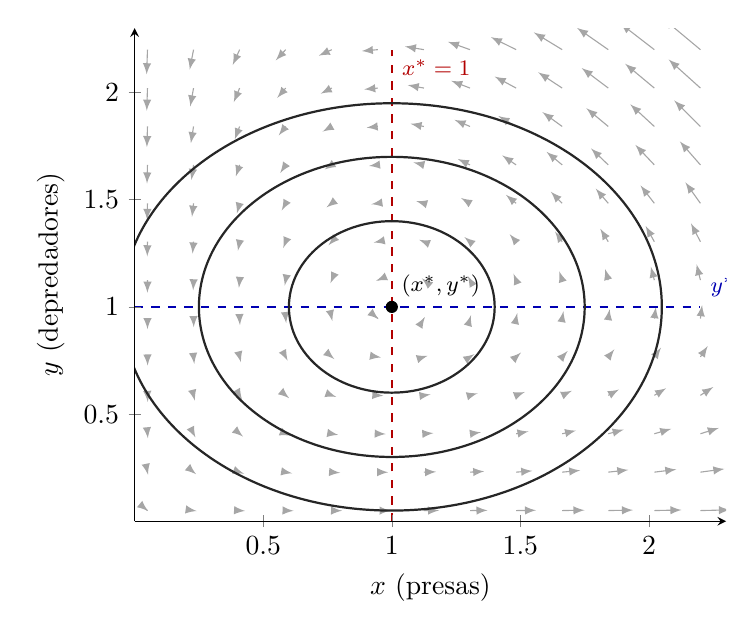
\begin{tikzpicture}
    \begin{axis}[
        view={0}{90}, domain=0.05:2.2, y domain=0.05:2.2,
        xmin=0, xmax=2.3, ymin=0, ymax=2.3,
        samples=13, width=0.75\linewidth,
        xlabel={$x$ (presas)}, ylabel={$y$ (depredadores)},
        axis lines=middle, grid=both, grid style={gray!15},
        xlabel near ticks, ylabel near ticks,
      ]
      \addplot3[gray!70, -latex, quiver={
          u={x - x*y}, v={-y + x*y}, scale arrows=0.055}] (x,y,0);
      \draw[red!70!black, thick, dashed] (axis cs:1,0) -- (axis cs:1,2.2)
        node[below right, font=\footnotesize]{$x^{*}=1$};
      \draw[blue!70!black, thick, dashed] (axis cs:0,1) -- (axis cs:2.2,1)
        node[above right, font=\footnotesize]{$y^{*}=1$};
      
      % Curvas de nivel cerradas de V(x,y) = x - ln x + y - ln y
      \draw[thick, black!85] (axis cs:1,1) circle [x radius=0.4, y radius=0.4];
      \draw[thick, black!85] (axis cs:1,1) circle [x radius=0.75, y radius=0.7];
      \draw[thick, black!85] (axis cs:1,1) circle [x radius=1.05, y radius=0.95];

      \fill (axis cs:1,1) circle (2.2pt) node[above right, font=\footnotesize]{$(x^{*},y^{*})$};
    \end{axis}
  \end{tikzpicture}
  \caption{Retrato de fases del modelo de Lotka--Volterra con $\alpha=\beta=\gamma=\delta=1$. Las líneas discontinuas representan las nullclines ($x^*=1, y^*=1$) y las curvas cerradas concéntricas son las trayectorias periódicas generadas por la integral primera $V(x,y) = C$.}
  \label{fig:lv_phase}
\end{figure}

\subsection{Simulación computacional: Python y NetLogo}

\paragraph{Integración numérica en Python.}
El sistema~\eqref{eq:lv-x}--\eqref{eq:lv-y} puede integrarse numéricamente de forma directa mediante esquemas estándar como Euler o Runge--Kutta:

\begin{minted}[fontsize=\small, framesep=4pt, frame=lines]{python}
import numpy as np

alpha, beta, gamma, delta = 1.0, 1.0, 1.0, 1.0

def lv(u, t):
    """Campo vectorial de Lotka-Volterra."""
    x, y = u
    return np.array([alpha*x - beta*x*y,
                     -gamma*y + delta*x*y])

dt, T = 0.01, 20.0        # paso temporal y horizonte
u = np.array([1.2, 0.6])  # condición inicial
for t in np.arange(0, T, dt):
    u = u + dt * lv(u, t)
print(f"estado final: x = {u[0]:.3f}, y = {u[1]:.3f}")
\end{minted}

\paragraph{Simulación basada en agentes en NetLogo.}
La misma dinámica poblacional puede explorarse a nivel individual en un modelo basado en agentes~\cite{netlogo}, donde cada presa y depredador es una tortuga discreta con reglas de búsqueda, alimentación y reproducción:

\begin{minted}[fontsize=\small, framesep=4pt, frame=lines]{lexer/netlogo.py:NetLogoLexer}
globals [presas-iniciales depredadores-iniciales]
turtles-own [energia]

to setup
  clear-all
  create-turtles presas-iniciales [
    setxy random-xcor random-ycor
    set color green  set energia 10
  ]
  create-turtles depredadores-iniciales [
    setxy random-xcor random-ycor
    set color red
  ]
  reset-ticks
end

to go
  ask turtles [
    ifelse color = red
      [ let presa min-one-of turtles with [color = green]
                        [distance-to self]
        if presa != nobody [ face presa  fd 1.2 ] ]
      [ fd 1  set energia energia - 1
        if energia < 2 [ die ] ]
  ]
  tick
end
\end{minted}

\paragraph{Conexión con tiempo discreto: mapa logístico y caos.}
Si en lugar de tiempo continuo se modela la población con generaciones discretas no superpuestas $N_{t+1} = r N_t (1 - N_t/K)$~\cite{may1976}, aparece el célebre mapa logístico cuadrático. Como demostró Robert May en 1976, al incrementar la tasa de crecimiento intrínseca el sistema pasa por una cascada infinita de duplicación de periodos y desemboca en caos determinista, ilustrando la riqueza que adquieren las no linealidades en dominios iterados.

\subsection{Centros vs Ciclos Límite: Estabilidad estructural}

A pesar de su elegancia histórica, el modelo de Lotka--Volterra adolece de una severa limitación desde el punto de vista biológico: es \textbf{estructuralmente inestable}~\cite{strogatz2015,murray2002}.

En un centro conservativo como el de Lotka--Volterra:
\begin{enumerate}
    \item La amplitud y el periodo de la oscilación dependen por completo de la condición inicial $(x_0, y_0)$.
    \item Si una perturbación ambiental transitoria desplaza al sistema (por ejemplo, una sequía que diezme momentáneamente las presas), el sistema salta a una órbita cerrada diferente y \textbf{jamás regresa a la oscilación original}. No existe ninguna fuerza restauradora sobre la amplitud.
    \item Cualquier modificación biológicamente realista ---como agregar una capacidad de carga $K$ para las presas ($\dot{x} = \alpha x (1 - x/K) - \beta x y$) o una respuesta funcional de saturación de Holling tipo II--- destruye inmediatamente el centro, convirtiéndolo en un foco espiral amortiguado o en un ciclo límite.
\end{enumerate}

Los osciladores biológicos reales (el marcapasos del nódulo sinoauricular del corazón, las oscilaciones circadianas de proteínas \emph{Clock/Period}, el ritmo respiratorio) no funcionan como centros frágiles: son notablemente robustos. Si el corazón sufre una perturbación (un sobresalto o una arritmia transitoria), la trayectoria es atraída de regreso al mismo ritmo y a la misma amplitud exacta. Este comportamiento no es un centro, sino un \textbf{ciclo límite atractor}.

\begin{definition}[Ciclo Límite]
Un \textbf{ciclo límite} $\Gamma$ es una trayectoria periódica cerrada e \textbf{aislada} en el espacio de fases de un sistema continuo. El término \emph{aislado} significa que en una vecindad tubular de $\Gamma$ no existen otras órbitas cerradas:
\begin{itemize}
    \item \textbf{Estable (atractor):} Todas las trayectorias vecinas espiralan hacia $\Gamma$ cuando $t \to +\infty$.
    \item \textbf{Inestable (repulsor):} Todas las trayectorias vecinas se alejan de $\Gamma$ cuando $t \to +\infty$.
    \item \textbf{Semi-estable:} Las trayectorias se aproximan a $\Gamma$ por un lado y se alejan por el otro.
\end{itemize}
\end{definition}

\subsection{El oscilador de Van der Pol y osciladores biológicos}

El prototipo fundamental de un oscilador no lineal con ciclo límite fue formulado en 1926 por el ingeniero y físico holandés Balthasar van der Pol para describir circuitos con tubos de vacío (tríodos) y, posteriormente, para modelar el ritmo autónomo del corazón humano:
\begin{equation}
    \ddot{x} - \mu (1 - x^2)\dot{x} + x = 0, \quad \mu > 0.
    \label{eq:vanderpol_ode}
\end{equation}
Escribiendo en variables de estado $(x, y = \dot{x})$:
\begin{equation}
\begin{aligned}
    \dot{x} &= y, \\
    \dot{y} &= -x + \mu(1 - x^2)y.
\end{aligned}
\label{eq:vanderpol_sistema}
\end{equation}

\paragraph{Mecanismo físico de disipación no lineal.}
El término $-\mu(1 - x^2)\dot{x}$ actúa como un coeficiente de amortiguamiento dependiente del estado:
\begin{itemize}
    \item Para pequeñas amplitudes ($|x| < 1$): El coeficiente es negativo ($-\mu(1-x^2) < 0$). El sistema experimenta amortiguamiento negativo, inyectando energía y amplificando cualquier perturbación lejos del origen inestable.
    \item Para grandes amplitudes ($|x| > 1$): El coeficiente es positivo ($+\mu(x^2-1) > 0$). El sistema disipa energía, frenando la oscilación.
\end{itemize}
El balance dinámico exacto entre la inyección de energía para $|x| < 1$ y la disipación para $|x| > 1$ fuerza la existencia de una única órbita periódica cerrada aislada de amplitud finita $x_{\max} \approx 2$: el \textbf{ciclo límite de Van der Pol} (véase la \cref{fig:vanderpol_portrait}).

\begin{figure}[htbp]
\centering
\begin{tikzpicture}[>=Stealth, scale=0.95]
    \begin{axis}[
        xmin=-3.2, xmax=3.2, ymin=-3.5, ymax=3.5,
        axis lines=middle,
        xlabel={$x$}, ylabel={$y = \dot{x}$},
        xlabel style={at={(ticklabel* cs:1)},anchor=west},
        ylabel style={at={(ticklabel* cs:1)},anchor=south},
        width=0.82\linewidth, height=6.8cm,
        grid=both, grid style={gray!20}
    ]
        % Ciclo límite de Van der Pol para mu=1 (aproximación numérica suave)
        \draw[very thick, black!95] plot [smooth cycle, tension=0.8] coordinates {
            (2.0, 0) (1.8, 1.2) (0.8, 2.2) (-0.5, 2.5) (-2.0, 0.2)
            (-1.8, -1.2) (-0.8, -2.2) (0.5, -2.5) (1.9, -0.2)
        };

        % Trayectoria espiral interna que sale del origen y converge al ciclo límite
        \draw[thick, black!65, domain=0:12.56, samples=150, variable=\t]
            plot ({ (0.2 + 0.14*\t)*cos(\t r) }, { (0.2 + 0.14*\t)*sin(\t r) });

        % Trayectoria exterior que entra al ciclo límite
        \draw[thick, black!65, domain=0:8.0, samples=120, variable=\t]
            plot ({ (3.0 - 0.12*\t)*cos(\t r) }, { (3.0 - 0.12*\t)*sin(\t r) });

        % Origen inestable
        \draw[black, fill=white, thick] (axis cs:0,0) circle (2.5pt) node[below right=2pt, font=\tiny] {Foco inestable};

        % Flecha de convergencia
        \node[font=\bfseries\footnotesize, fill=white, inner sep=1pt] at (axis cs:1.4, 2.6) {Ciclo límite $\Gamma$};
        \node[font=\footnotesize, black!75] at (axis cs:-2.0, -2.8) {Atractor asintótico global en $\mathbb{R}^2 \setminus \{\vec{0}\}$};
    \end{axis}
\end{tikzpicture}
\caption{Retrato de fases del oscilador de Van der Pol con $\mu = 1$. El origen es un foco inestable que repele las trayectorias; todas las soluciones (interiores y exteriores) son atraídas asintóticamente hacia el ciclo límite aislado $\Gamma$.}
\label{fig:vanderpol_portrait}
\end{figure}

\paragraph{Universalidad biológica de los ciclos límite.}
Como anticipamos en la introducción histórica del curso (capítulo 2), los ciclos límite son la base teórica de:
\begin{itemize}
    \item \textbf{Marcapasos cardíacos:} El potencial de membrana de las células marcapasos oscila espontáneamente sin necesidad de estímulo externo.
    \item \textbf{Excitabilidad neuronal:} El modelo de FitzHugh--Nagumo (una simplificación bidimensional del sistema de 4 variables de Hodgkin--Huxley) utiliza la geometría tipo Van der Pol para explicar cómo una neurona pasa del reposo a la emisión periódica de espigas (\emph{spiking}).
    \item \textbf{Relojes circadianos y biológicos:} Arthur Winfree~\cite{winfree2001} demostró que la geometría de fases de los ciclos límite permite entender la sincronización y el desfase (\emph{jet lag}) de los ritmos biológicos circadianos bajo pulsos de luz externos.
\end{itemize}

% integrado de body/body.tex
